\usetikzlibrary{arrows.meta,decorations.pathmorphing,decorations.pathreplacing}
\begin{frame}{blocking signals}
\begin{itemize}
\item avoid having signal handlers anywhere:
\item can instead \myemph{block signals}
    \begin{itemize}
    \item \texttt{sigprocmask()}, \texttt{pthread\_sigmask()}
    \end{itemize}
\item blocked = signal handler doesn't run
    \begin{itemize}
    \item also called ``masking'' a signal
    \item blocked signals are not \textit{delivered} (acted on)
    \end{itemize}
\item instead, signal becomes \textit{pending}
    \begin{itemize}
    \item delivered if unblocked
    \end{itemize}
\end{itemize}
\begin{tikzpicture}[overlay,remember picture]
\begin{visibleenv}<2->
\coordinate (base) at ([xshift=-2cm,yshift=-1cm]current page.north east);
\draw[very thick,decoration={snake},decorate,-Latex] (base) -- ++(0cm, -8cm) coordinate (snake bottom);
\draw[thick,dotted] ([yshift=-.5cm]base) -- ++(-.5cm,0cm) node[font=\small,align=right,left] (block)
    {block signal};
\draw[thick,dotted] ([yshift=-3cm]base) -- ++(-.5cm,0cm) node[font=\small,align=right,left] {receive\\signal};
\draw[violet,very thick,decoration={brace},decorate] ([yshift=-.5cm,xshift=.25cm]base) -- ++(0cm,-2.5cm)
    node[midway,right] {blocked};
\draw[red,ultra thick,decoration={brace},decorate] ([yshift=-3cm,xshift=.25cm]base) -- ++(0cm,-3cm)
    node[midway,right,align=left] {blocked \\ and \\pending};

\draw[thick,dotted] ([yshift=-6cm]base) -- ++(-.5cm,.15cm) node[font=\small,align=right,left] {unblock signal};
\draw[thick,dotted] ([yshift=-6cm]base) -- ++(-.5cm,-.15cm) node[font=\small,align=right,left] {signal handler runs};
\end{visibleenv}
\end{tikzpicture}
\end{frame}

\begin{frame}{controlling when signals are handled}
\begin{itemize}
\item first, block a signal
\item then either unblock signals only at certain times
    \begin{itemize}
        \item some special functions to help: \\ {\tt sigsuspend} (unblock and wait until handler runs), \\ {\tt pselect} (unblock while checking for I/O), \ldots
    \end{itemize}
\item and/or use API for checking/changing pending signals
    \begin{itemize}
    \item example: \myemph<2>{{\tt sigwait}} \\
        (wait for blocked signal to become pending; \\
        then mark not pending)
    \item typically \myemph{instead of having signal handler}
    \end{itemize}
\end{itemize}
\begin{tikzpicture}[overlay,remember picture]
\coordinate (base) at ([xshift=-2cm,yshift=-1cm]current page.north east);
\draw[very thick,decoration={snake},decorate,-Latex] (base) -- ++(0cm, -8cm);
\draw[thick,dotted] ([yshift=-.5cm]base) -- ++(-.5cm,0cm) node[font=\small,align=right,left] (block)
    {block signal};
\draw[thick,dotted] ([yshift=-3cm]base) -- ++(-.5cm,0cm) node[font=\small,align=right,left] {receive\\signal};
\draw[violet,very thick,decoration={brace},decorate] ([yshift=-.5cm,xshift=.25cm]base) -- ++(0cm,-2.5cm)
    node[midway,right] {blocked};
\draw[red,ultra thick,decoration={brace},decorate] ([yshift=-3cm,xshift=.25cm]base) -- ++(0cm,-2cm)
    node[midway,right,align=left] {blocked \\ and \\pending};
\draw[violet,very thick,decoration={brace},decorate] ([yshift=-5cm,xshift=.25cm]base) -- ++(0cm,-1cm)
    node[midway,right,align=left] {blocked};
\draw[thick,dotted] ([yshift=-5cm]base) -- ++(-.5cm,.15cm) node[font=\small,align=right,left] {sigwait};
\draw[violet,very thick,decoration={brace},decorate] ([yshift=-.5cm,xshift=.25cm]base) -- ++(0cm,-2.5cm)
    node[midway,right] {blocked};
\draw[thick,dotted] ([yshift=-6cm]base) -- ++(-.5cm,.15cm) node[font=\small,align=right,left] {unblock signal};
\end{tikzpicture}
\end{frame}

\begin{frame}{sigwait timelines}
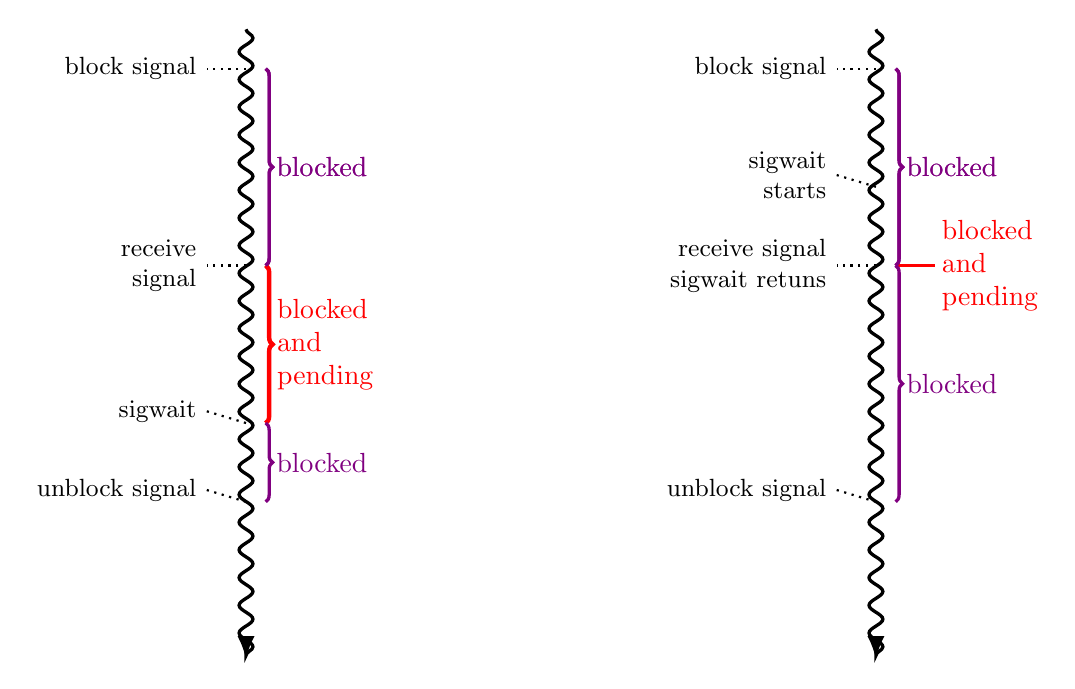
\begin{tikzpicture}
\coordinate (base) at (0, 0);
\draw[very thick,decoration={snake},decorate,-Latex] (base) -- ++(0cm, -8cm);
\draw[thick,dotted] ([yshift=-.5cm]base) -- ++(-.5cm,0cm) node[font=\small,align=right,left] (block)
    {block signal};
\draw[thick,dotted] ([yshift=-3cm]base) -- ++(-.5cm,0cm) node[font=\small,align=right,left] {receive\\signal};
\draw[violet,very thick,decoration={brace},decorate] ([yshift=-.5cm,xshift=.25cm]base) -- ++(0cm,-2.5cm)
    node[midway,right] {blocked};
\draw[red,ultra thick,decoration={brace},decorate] ([yshift=-3cm,xshift=.25cm]base) -- ++(0cm,-2cm)
    node[midway,right,align=left] {blocked \\ and \\pending};
\draw[violet,very thick,decoration={brace},decorate] ([yshift=-5cm,xshift=.25cm]base) -- ++(0cm,-1cm)
    node[midway,right,align=left] {blocked};
\draw[thick,dotted] ([yshift=-5cm]base) -- ++(-.5cm,.15cm) node[font=\small,align=right,left] {sigwait};
\draw[violet,very thick,decoration={brace},decorate] ([yshift=-.5cm,xshift=.25cm]base) -- ++(0cm,-2.5cm)
    node[midway,right] {blocked};
\draw[thick,dotted] ([yshift=-6cm]base) -- ++(-.5cm,.15cm) node[font=\small,align=right,left] {unblock signal};

\begin{scope}[shift={(8, 0)},name prefix=shifted-]
\coordinate (base) at (0, 0);
\draw[very thick,decoration={snake},decorate,-Latex] (base) -- ++(0cm, -8cm);
\draw[thick,dotted] ([yshift=-.5cm]base) -- ++(-.5cm,0cm) node[font=\small,align=right,left] (block)
    {block signal};
\draw[violet,very thick,decoration={brace},decorate] ([yshift=-.5cm,xshift=.25cm]base) -- ++(0cm,-2.5cm)
    node[midway,right] {blocked};
\draw[thick,dotted] ([yshift=-2cm]base) -- ++(-.5cm,.15cm) node[font=\small,align=right,left] {sigwait\\starts};
\draw[thick,dotted] ([yshift=-3cm]base) -- ++(-.5cm,0cm) node[font=\small,align=right,left] {receive signal\\sigwait retuns};
\draw[red,very thick] ([yshift=-3cm,xshift=.25cm]base) --++(.5cm, 0cm)
    node[xshift=.2cm,midway,right,align=left] {blocked\\and\\ pending};
\draw[violet,very thick,decoration={brace},decorate] ([yshift=-3cm,xshift=.25cm]base) -- ++(0cm,-3cm)
    node[midway,right,align=left] {blocked};
\draw[violet,very thick,decoration={brace},decorate] ([yshift=-.5cm,xshift=.25cm]base) -- ++(0cm,-2.5cm)
    node[midway,right] {blocked};
\draw[thick,dotted] ([yshift=-6cm]base) -- ++(-.5cm,.15cm) node[font=\small,align=right,left] {unblock signal};
\end{scope}
\end{tikzpicture}
\end{frame}

\begin{frame}[fragile,label=syncSig]{synchronous signal handling}
\lstset{language=C,style=small}
\begin{lstlisting}
int main(void) {
    sigset_t set;
    sigemptyset(&set);
    sigaddset(&set, SIGINT);
    sigprocmask(SIG_BLOCK, &set, NULL);
    
    printf("Waiting for SIGINT (control-C)\n"); 
    int num;
    if (sigwait(&set, &num) != 0) {
        printf("sigwait failed!\n");
    }
    if (num == SIGINT);
        printf("Got SIGINT\n");
    }
}
\end{lstlisting}
\end{frame}

